% !TEX program = xelatex
\documentclass[10pt,letterpaper]{article}

\usepackage[T1]{fontenc}
\usepackage{lmodern}
\usepackage[top=0.72in,bottom=0.78in,left=0.82in,right=0.82in]{geometry}
\usepackage{microtype}
\usepackage{graphicx}
\usepackage{booktabs}
\usepackage{tabularx}
\usepackage{array}
\usepackage{multirow}
\usepackage{amsmath,amssymb}
\usepackage{tikz}
\usetikzlibrary{arrows.meta,positioning,fit,calc}
\usepackage{enumitem}
\usepackage{xspace}
\usepackage{xcolor}
\usepackage{caption}
\usepackage{subcaption}
\usepackage{placeins}
\usepackage{float}
\usepackage{fancyhdr}
\usepackage{titlesec}
\usepackage[numbers,sort&compress]{natbib}
\usepackage{hyperref}
\usepackage[capitalise,noabbrev]{cleveref}

\definecolor{navy}{HTML}{17365D}
\definecolor{linkblue}{HTML}{1D4ED8}
\definecolor{softgray}{HTML}{F3F6F9}
\definecolor{rulegray}{HTML}{CBD5E1}

\hypersetup{
  colorlinks=true,
  linkcolor=navy,
  citecolor=linkblue,
  urlcolor=linkblue,
  pdftitle={ElasticUMA: Reload-Correct OS-Managed Expert Caching for Apple Silicon},
  pdfauthor={Naresh Prajapati},
  pdfsubject={Apple Silicon mixture-of-experts inference systems},
  pdfkeywords={Apple Silicon, unified memory, mixture of experts, Metal, purgeable memory}
}

\titleformat{\section}{\Large\bfseries\color{navy}}{\thesection}{0.55em}{}
\titleformat{\subsection}{\large\bfseries\color{navy}}{\thesubsection}{0.5em}{}
\titleformat{\subsubsection}{\normalsize\bfseries}{\thesubsubsection}{0.45em}{}
\titlespacing*{\section}{0pt}{1.35em}{0.45em}
\titlespacing*{\subsection}{0pt}{1.05em}{0.35em}
\titlespacing*{\subsubsection}{0pt}{0.8em}{0.25em}

\captionsetup{
  font=small,
  labelfont={bf,color=navy},
  textfont=small,
  justification=justified,
  singlelinecheck=false,
  skip=5pt
}
\setlist[itemize]{leftmargin=1.35em,itemsep=0.15em,topsep=0.3em}
\setlist[enumerate]{leftmargin=1.55em,itemsep=0.15em,topsep=0.3em}
\setlength{\parindent}{1.05em}
\setlength{\parskip}{0pt}
\setlength{\textfloatsep}{12pt plus 2pt minus 3pt}
\setlength{\floatsep}{10pt plus 2pt minus 2pt}
\setlength{\intextsep}{10pt plus 2pt minus 2pt}
\renewcommand{\topfraction}{0.92}
\renewcommand{\bottomfraction}{0.85}
\renewcommand{\textfraction}{0.06}
\renewcommand{\floatpagefraction}{0.82}
\setcounter{topnumber}{3}
\setcounter{bottomnumber}{2}
\setcounter{totalnumber}{4}
\emergencystretch=1em

\pagestyle{fancy}
\fancyhf{}
\fancyhead[L]{\small\sffamily ElasticUMA}
\fancyhead[R]{\small\sffamily Author Preprint}
\fancyfoot[C]{\small\thepage}
\renewcommand{\headrulewidth}{0.35pt}
\setlength{\headheight}{14pt}

\newcommand{\system}{ElasticUMA\xspace}
\newcommand{\gib}{\,GiB\xspace}
\newcommand{\mib}{\,MiB\xspace}
\newcommand{\tps}{\,token/s\xspace}
\newcommand{\code}[1]{\texttt{#1}}
\newcommand{\artifacthash}[1]{\nolinkurl{#1}}
\newcommand{\yes}{\textbf{yes}}
\newcommand{\no}{\textbf{no}}

\title{ElasticUMA: Reload-Correct OS-Managed Expert Caching for Apple Silicon}
\author{Naresh Prajapati}
\date{}

\begin{document}
\thispagestyle{empty}

\begin{center}
  {\fontsize{18}{22}\selectfont\bfseries\color{navy}
  ElasticUMA: Reload-Correct OS-Managed\\[-1pt]
  Expert Caching for Apple Silicon\par}
  \vspace{0.65em}
  {\large\bfseries Naresh Prajapati\par}
  \vspace{0.18em}
  {\normalsize Independent Researcher\par}
  \vspace{0.12em}
  {\small\href{mailto:prajapatinaresh084.pn@gmail.com}{prajapatinaresh084.pn@gmail.com}\par}
  \vspace{0.4em}
  {\small Code and artifact: \url{https://github.com/Naresh084/elasticuma}\par}
\end{center}
\vspace{0.25em}
\noindent\color{rulegray}\rule{\linewidth}{0.7pt}\color{black}

\begin{abstract}
Storage-backed MoE inference on Apple Silicon has a shared-memory problem: one
physical pool serves the CPU, GPU, filesystem cache, applications, compressor,
and swap. For storage-backed
mixture-of-experts (MoE) inference, a large explicit expert cache can therefore
raise its local hit rate while increasing system pressure and reducing
end-to-end throughput. This paper introduces \system, a reload-correct expert
cache that separates logical capacity from physical entitlement. Each expert
slot is a Metal-owned shared buffer. The runtime keeps a small hot set
nonvolatile and marks cold slots volatile only at synchronized prefill-layer and
decode-token boundaries. Before treating a volatile mapping as a hit, it
relocks the buffer. If Metal reports that the contents are empty, \system
invalidates the mapping and reloads the exact expert bytes before GPU binding.

We evaluate the committed mechanism against untouched fixed-16 and fixed-96
upstream policies on an M1 Max with 32\,GiB unified memory. Under a bounded
4\,GiB co-tenant, Qwen3.6-35B-A3B Q4 gains 7.25\% and 13.67\% paired-median
decode throughput over the two baselines, while reducing fixed-96 peak physical
footprint by 31.64\%. Without synthetic pressure, the gains are 16.91\% and
17.59\%, with a 31.65\% footprint reduction. A second architecture, Gemma 4
26B-A4B Q4, gains 45.30\% and 26.01\% and reduces fixed-96 footprint by
35.26\%. All 45 positive measured rows pass admission with within-protocol
output equality and observed empty-slot recovery. The contribution is a
two-architecture mechanism on one Mac that lets a large logical cache coexist
with OS-wide reclamation; it does not establish cross-generation, energy,
concurrency, or independent-reproduction claims.
\end{abstract}

\noindent\textbf{Keywords:} Apple Silicon, unified memory,
mixture-of-experts inference, Metal, purgeable memory, expert caching.

\section{Introduction}
\label{sec:introduction}

Open-weight mixture-of-experts (MoE) models decouple total model capacity from
the computation performed for each token. A router selects a small subset of
experts, so a model with tens or hundreds of billions of parameters may execute
only a few billion active parameters at a time. That sparsity makes local
serving possible, but it does not make the inactive weights disappear. A local
runtime must still place the complete expert pool and move requested experts
into execution memory. It must also decide which cached state should survive
when the machine becomes busy.

FreeToken addresses this problem on heterogeneous CUDA systems by combining a
host-resident expert pool, a GPU expert cache, double-buffered prefill, and a
bandwidth-calibrated choice between CPU execution and PCIe transfer
\cite{yang2026freetoken}. KTransformers similarly demonstrates that CPU-GPU
hybrid execution can make large MoE checkpoints practical on commodity
machines \cite{chen2025ktransformers}. These systems exploit a resource model
with distinct host and device memories. Apple Silicon changes that model. The
CPU and GPU share physical memory, and Metal shared buffers do not cross a PCIe
boundary. Expert slots, immutable file-backed weights, prompt state, the
filesystem cache, the display stack, desktop applications, compression, and
swap all compete in the same pool.

This shared pool creates a failure mode that is invisible to cache-local
metrics. We first characterize whether cache hit rate tracks end-to-end service
performance. Increasing explicit expert capacity can raise the hit rate yet
evict useful file-backed pages, increase compression, and reduce decode speed.
Our preregistered fixed-cache sweep demonstrates that tension. Increasing Qwen
from 16 to 96 expert slots per layer raises median hit rate from 48.98\% to
90.13\%, while median decode throughput falls from 11.330 to 10.120\tps. Peak
compressor growth also increases by roughly 5\gib. The paired slowdown is
10.54\%, below the frozen 15\% threshold required to authorize our original
cache-size controller. We retain that negative result and abandon the
controller rather than lower its gate.

The fixed-cache curve suggests a different mechanism. The runtime benefits from
the logical identity and reuse information of a large cache, but it need not
claim permanent physical residency for every cold slot. Apple exposes
purgeable Metal resources for exactly this cache-like relationship: an
application may mark a resource volatile, the operating system may reclaim its
contents, and the application must relock and recreate or reload the resource
before access \cite{apple2026purgeable,apple2026metalfootprint}. Applying that
contract to model weights is not automatic. A cache mapping can outlive the
physical contents it names; a GPU command may still reference a resource when a
state transition is attempted; and externally allocated memory wrapped by
Metal may remain physically owned even when the wrapper is marked purgeable.

We present \system to resolve those correctness and integration problems. Each
expert slot is allocated through Metal and retains a stable CPU pointer for
positional reads. The cache tracks each slot as nonvolatile, volatile, or
empty. At safe boundaries it
keeps the hottest slots nonvolatile and offers the cold remainder to macOS. A
future logical hit is provisional until a nonvolatile relock confirms that its
contents survived. An empty return clears identity and recency state and enters
the existing exact miss path. The GPU sees either validated cached bytes or a
fully reloaded expert; discarded contents cannot reach a command encoder.

This paper makes four contributions:

\begin{itemize}
  \item It characterizes the mismatch between expert-cache hit rate and
  end-to-end service performance in one Apple unified-memory system, including
  a preregistered negative result that stops an earlier controller claim.
  \item It presents a reload-correct state machine for Metal-owned expert slots,
  with explicit validity, publication, and GPU-synchronization invariants.
  \item It integrates selective purgeability at the actual prefill-layer and
  decode-token boundaries, avoiding the full physical prefill peak that defeats
  a post-prefill-only policy.
  \item It evaluates the committed implementation against untouched small- and
  large-cache upstream binaries on Qwen3.6 and Gemma 4, with balanced held-out
  repetitions, physical-footprint telemetry, exact-recovery receipts, negative
  alternatives, immutable artifacts, and explicit claim limits.
\end{itemize}

The strongest supported conclusion is intentionally scoped. On the measured M1
Max workloads, \system improves the throughput-footprint frontier: it dominates
fixed-96 with higher throughput and lower footprint, while providing more
throughput and locality than fixed-16 at a higher footprint. One host and two
architectures do not establish an all-Mac result. Cross-chip reproduction,
energy measurement, longer contexts, concurrency, and independent operation
remain required.

\section{Background and Motivation}
\label{sec:background}

\subsection{Storage-backed routed-expert inference}

An MoE layer contains a router, a shared or dense path, and a pool of routed
experts. For each token the router selects a small top-$k$ set. A bounded-memory
runtime can keep non-expert tensors resident while reading selected expert
tensors from storage into a fixed number of execution slots. MoE-Infinity shows
that request-level sparsity and expert reuse support prefetching and caching on
personal machines \cite{xue2024moeinfinity}. MawForge demonstrates a related
storage-backed design on constrained unified-memory systems and finds that
maximum cache capacity is not itself an optimal policy \cite{opie2026mawforge}.

The executor used in this study descends from slipstream
\cite{patel2026slipstream}. It stores immutable layer files in a packed
\code{.gturbo} directory, maintains a bounded per-layer routed-expert cache,
loads misses with positional reads, and executes native Metal kernels. The
upstream fixed policy owns every allocated slot until the model unloads. This
provides a strong controlled baseline because the model, quantization, kernels,
tokenizer, storage layout, and request path remain constant while cache
residency changes.

\subsection{Why Apple unified memory is not free capacity}

Unified addressing removes explicit host-to-device copies, but it does not
remove physical scarcity. The same DRAM services CPU and GPU demand, file-backed
pages, anonymous allocations, and the compressor. A process's resident set size
also becomes an unreliable measure of its current physical claim: a purgeable
page may remain mapped and counted in RSS while the operating system is free to
discard its contents. We therefore use \code{proc\_pid\_rusage().ri\_phys\_footprint}
as the primary process metric and report RSS only as secondary context.

Apple documents \code{MTLPurgeableState.volatile} as a cache state whose
contents may be discarded, and \code{setPurgeableState} returns the prior state
when an application relocks a resource \cite{apple2026purgeable}. This creates
two distinct notions of capacity:

\begin{itemize}
  \item \textbf{Logical capacity} is the number of expert identities and stable
  Metal resources represented by the cache.
  \item \textbf{Physical entitlement} is the subset of pages the application
  currently insists must remain valid.
\end{itemize}

A fixed cache equates the two. \system deliberately separates them.

\subsection{Prefill and decode expose different residency shapes}

Prompt prefill processes many tokens in parallel and often activates a broad
union of experts. Decode processes one new token at a time and exhibits stronger
short-range route reuse. FreeToken treats these phases differently through
full-layer streaming in prefill and semantic-aware caching in decode
\cite{yang2026freetoken}. The phase distinction is also necessary on Apple UMA,
but for a different reason. If cold slots become volatile only after all
prefill completes, every layer can materialize its large cache first. The host
has already paid the peak physical cost before the policy runs. \system must
offer cold pages to the OS immediately after each layer's routed GPU work
finishes.

\subsection{The rejected cache-size controller}

Our initial hypothesis was that a live pressure signal could select among fixed
cache sizes. We froze a 15\% throughput-gap gate before measuring Qwen. The
fixed sweep found a stable 10.54\% paired slowdown from 16 to 96 slots, with
five of five pairs in the same direction, but it did not reach the gate. This
result has two implications. First, the pressure tradeoff is real but not large
enough to justify a controller built around ordinary cache-size switching.
Second, changing the threshold after observing the data would turn a
falsification gate into post-hoc selection. We instead test a new mechanism
with new prompts, new experiment identifiers, and separately frozen gates.

\FloatBarrier

\begin{figure}[tb]
  \centering
  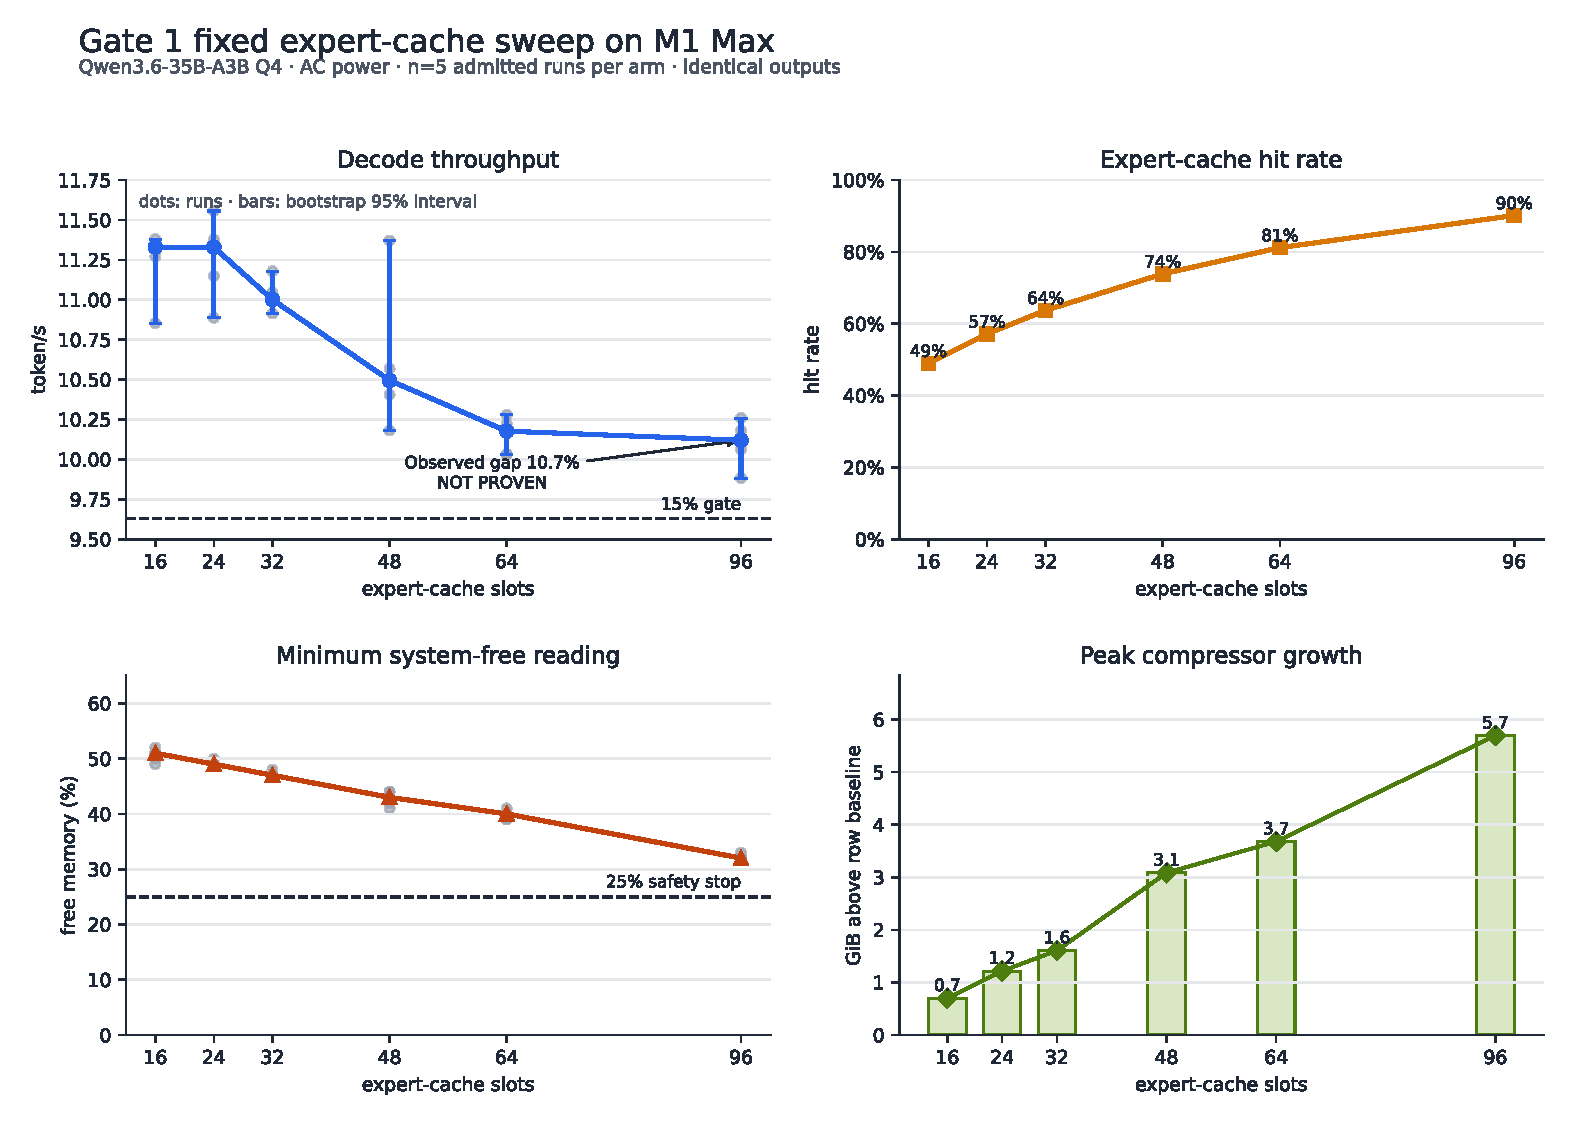
\includegraphics[width=0.98\linewidth]{figures/gate1-v4.pdf}
  \caption{Fixed-cache characterization on Qwen3.6-35B-A3B Q4. More slots
  monotonically raise hit rate but reduce decode throughput and free-memory
  headroom while increasing compressor growth. The observed 16-to-96 slowdown
  misses the preregistered 15\% controller-authorization gate. Bars and points
  summarize five admitted measured repetitions per arm.}
  \label{fig:gate1}
\end{figure}

\FloatBarrier

\section{ElasticUMA Design}
\label{sec:design}

\subsection{Design goals}

\system is guided by four goals.

\begin{enumerate}
  \item \textbf{Exactness.} Reclamation may change latency and I/O, but never
  routing, weights, generated semantics, or the bytes observed by a GPU kernel.
  \item \textbf{Stable resources.} Existing Metal bindings and CPU-side
  positional reads should not require per-miss resource allocation.
  \item \textbf{Timely physical elasticity.} Cold pages must become
  reclaimable before later prefill layers create the global physical peak.
  \item \textbf{Baseline isolation.} Fixed residency must bypass the new state
  machine, preserving an untouched behavioral comparison.
\end{enumerate}

\begin{figure}[H]
  \centering
  \resizebox{0.98\linewidth}{!}{%
  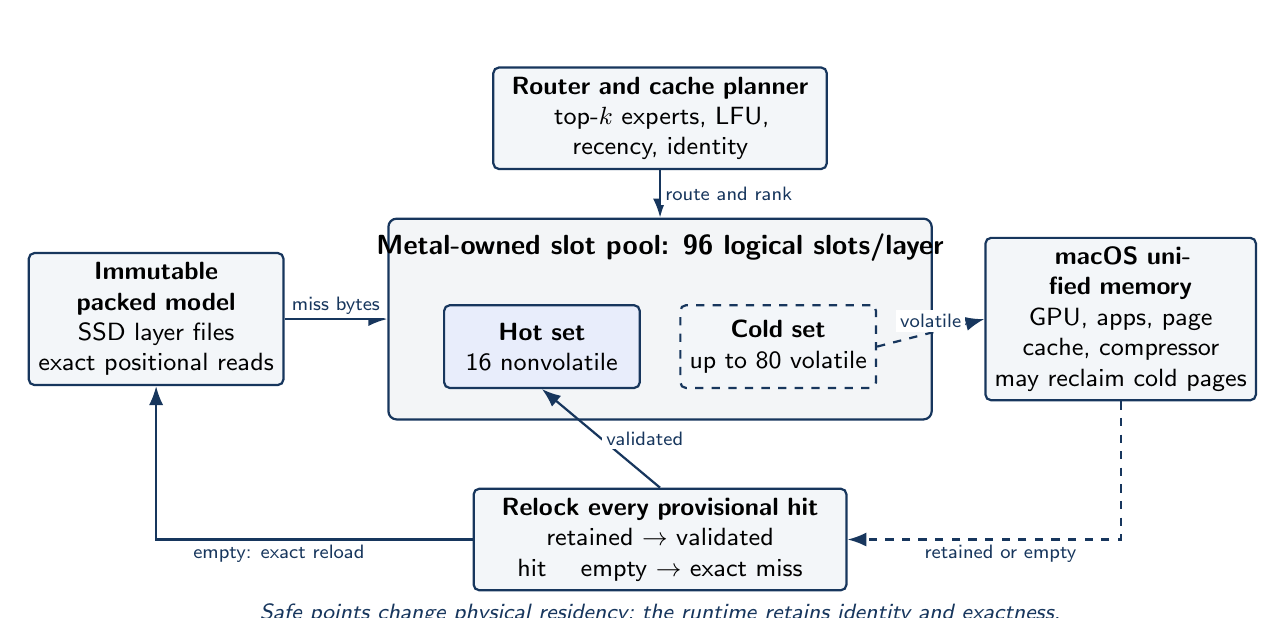
\begin{tikzpicture}[
    font=\sffamily\small,
    box/.style={draw=navy,thick,rounded corners=2pt,align=center,fill=softgray,minimum height=1.25cm},
    arrow/.style={-{Latex[length=2.4mm]},thick,draw=navy},
    darrow/.style={-{Latex[length=2.4mm]},thick,dashed,draw=navy},
    note/.style={font=\sffamily\scriptsize,align=center,fill=white,inner sep=1.5pt,text=navy}
  ]
    \node[box,text width=3.0cm] (store) at (2.0,1.7)
      {\textbf{Immutable packed model}\\SSD layer files\\exact positional reads};
    \node[box,text width=4.0cm] (planner) at (8.4,4.25)
      {\textbf{Router and cache planner}\\top-$k$ experts, LFU, recency, identity};
    \node[draw=navy,thick,rounded corners=3pt,fill=navy!5,
      minimum width=6.9cm,minimum height=2.55cm] (pool) at (8.4,1.7) {};
    \node[font=\sffamily\bfseries] at ($(pool.north)+(0,-0.38)$)
      {Metal-owned slot pool: 96 logical slots/layer};
    \node[box,fill=linkblue!10,text width=2.25cm,minimum height=1.05cm]
      (hot) at (6.9,1.35) {\textbf{Hot set}\\16 nonvolatile};
    \node[box,dashed,text width=2.25cm,minimum height=1.05cm]
      (cold) at (9.9,1.35) {\textbf{Cold set}\\up to 80 volatile};
    \node[box,text width=4.5cm] (relock) at (8.4,-1.10)
      {\textbf{Relock every provisional hit}\\retained $\rightarrow$ validated hit \quad empty $\rightarrow$ exact miss};
    \node[box,text width=3.2cm] (os) at (14.25,1.7)
      {\textbf{macOS unified memory}\\GPU, apps, page cache, compressor\\may reclaim cold pages};

    \draw[arrow] (planner.south) -- node[note,right]{route and rank} (pool.north);
    \draw[arrow] (store.east) -- node[note,above]{miss bytes} (pool.west);
    \draw[darrow] (cold.east) -- node[note,above]{volatile} (os.west);
    \draw[darrow] (os.south) |- node[note,below,pos=0.72]{retained or empty} (relock.east);
    \draw[arrow] (relock.west) -- ++(-0.9,0) -| node[note,below,pos=0.25]{empty: exact reload} (store.south);
    \draw[arrow] (relock.north) -- node[note,right]{validated} (hot.south);
    \node[note,fill=none,font=\sffamily\footnotesize\itshape] at (8.4,-2.05)
      {Safe points change physical residency; the runtime retains identity and exactness.};
  \end{tikzpicture}}
  \caption{\system separates logical cache identity from physical residency.
  The packed model is immutable. Hot Metal-owned slots remain nonvolatile;
  cold slots become volatile after GPU-safe boundaries. Every provisional hit
  is relocked. If macOS reports an empty prior state, the mapping is
  invalidated and exact bytes are reloaded before GPU use.}
  \label{fig:architecture}
\end{figure}

\FloatBarrier

\subsection{Metal-owned per-expert slots}

The upstream executor allocates anonymous CPU memory and wraps it in
\code{bytesNoCopy} Metal buffers. An isolated probe showed that making such a
wrapper purgeable does not surrender the external allocation: Metal does not
own the pages. \system instead allocates each slot with
\code{MTLDevice.makeBuffer(storageModeShared)} and uses the stable
\code{buffer.contents()} pointer as the destination of the existing exact
\code{pread} path. The Metal object and CPU pointer survive transitions among
nonvolatile, volatile, empty, and refilled states.

This choice is essential. Reallocating a resource on every empty recovery would
change binding identity, increase synchronization work, and complicate cache
publication. Stable Metal ownership lets physical contents disappear while the
runtime retains the slot object, its index, and its synchronization discipline.

\subsection{Residency and identity state}

For each slot $s$, the cache stores a Metal buffer $b_s$, an optional expert
identity $e_s$, LFU count $f_s$, recency timestamp $r_s$, and residency state
$q_s$. The state $q_s$ is one of:

\begin{center}
\begin{tabularx}{0.96\linewidth}{>{\bfseries}l X X}
\toprule
State & Physical contract & Valid use \\
\midrule
Nonvolatile & macOS must preserve contents & May be bound after normal cache planning \\
Volatile & macOS may discard contents & Must be relocked before a hit is accepted \\
Empty & Prior contents are invalid & Identity is cleared; exact reload is mandatory \\
\bottomrule
\end{tabularx}
\end{center}

Logical identity and physical validity may therefore diverge temporarily: a
volatile slot can still name expert $e_s$ even though macOS is allowed to
discard its bytes. The divergence is safe only because a volatile mapping is
provisional and cannot directly reach a GPU encoder.

\FloatBarrier

\subsection{Relock-before-hit protocol}

\Cref{tab:lookup} shows the lookup path. Planning runs under the same
cache lock that protects identity, LFU/recency data, residency state, and
recovery counters. A matching nonvolatile slot is an ordinary hit. A matching
volatile slot is first requested as nonvolatile. Metal returns the prior state:
retained contents preserve the hit, while an empty return invalidates the
mapping and turns the access into a miss. Before overwriting any volatile or
empty victim, the runtime also makes that buffer nonvolatile. Only a complete
positional read publishes the new expert identity.

\begin{table}[ht]
\centering
\caption{Reload-correct lookup for requested expert $e$. Every row executes
under the cache lock except the final GPU use.}
\label{tab:lookup}
\small
\begin{tabularx}{0.96\linewidth}{>{\bfseries}r X}
\toprule
1 & Find the slot $s$ whose published identity equals $e$, if one exists. \\
2 & If $s$ is volatile, request nonvolatile state and inspect the prior state. \\
3a & If contents were retained, record the relock and preserve the hit. \\
3b & If the prior state is empty, clear identity and validity and convert the access to a miss. \\
4 & On a validated hit, update LFU/recency and return the slot. \\
5 & On a miss, select a victim and make its Metal buffer nonvolatile. \\
6 & Read the complete expert blob positionally into the stable buffer pointer. \\
7 & Publish the new identity only after the complete read; then return the exact slot. \\
\bottomrule
\end{tabularx}
\end{table}

\FloatBarrier

\subsection{Selective hot and cold residency}

At a safe point, occupied slots are ranked first by cumulative use count and
then by recency. The configured hot subset remains nonvolatile. Every other
occupied nonvolatile slot transitions to volatile. The evaluated policy uses 96
logical slots and a 16-slot hot set per layer. This is not a claim that 16 is
universally optimal; it is a frozen policy chosen to combine the identity
capacity of the large cache with the physical commitment of a small working
set.

The OS remains free to keep volatile pages while memory is plentiful. Under
contention it can reclaim them without asking the model runtime to predict the
future. \system supplies model-specific admission, identity, and exact recovery;
macOS supplies global knowledge about competing physical demand.

\subsection{GPU-safe transition points}

Purgeability cannot change while a live command buffer may read a slot. During
chunked prefill, \system runs the residency policy after the just-completed
layer's routed tiles and tail command buffer finish. This lets layer $i$ offer
its cold pages before layer $i+1$ expands. During decode, the policy runs after
the complete step and output head finish. Both positions reuse synchronization
already required for router readback and command completion.

A post-prefill callback is insufficient. In an earlier implementation, every
layer reached its 96-slot physical peak before any slot became volatile. The
logical policy was correct but the peak-footprint gate failed. Moving the same
hot/cold transition into the layer loop changed when physical entitlement was
released and passed the successor gate.

\subsection{Correctness invariants}

The mechanism maintains five invariants:

\begin{enumerate}
  \item A GPU encoder binds a cached expert only when the slot is known
  nonvolatile.
  \item An empty prior state is never counted or consumed as a hit.
  \item A new expert identity is published only after a complete exact read.
  \item Purgeability transitions occur only after the last GPU command that may
  reference the affected resource has completed.
  \item Fixed mode executes none of the purgeability path.
\end{enumerate}

Together, the first four reduce OS reclamation to an ordinary exact cache miss.
The fifth preserves the baseline and provides a fail-safe mode on unsupported
systems.

\section{Implementation}
\label{sec:implementation}

The measured implementation is a 629-line change at runtime code commit
\code{ec84269d} over pinned upstream \code{01f7d5e7}. It is distributed as an
Apache-2.0 patch whose complete staged diff is verified before every public
build. The executable data path is Swift and Metal; Python is confined to model
installation, experiment orchestration, admission, and analysis.

\subsection{Cache and runner changes}

The patch replaces external slot storage with per-slot Metal-owned shared
buffers and adds the three-state residency field. It records volatile
transitions, relocks, retained relocks, empty recoveries, invalidated slots, and
cumulative recovered bytes. Cache lookup calls the relock path while holding
the cache lock. Recovery reuses the existing exact positional reader and does
not alter router scores or tensor representation.

The model layer exposes one call that applies the hot/cold policy to all routed
expert caches. The prefill runner invokes it after each synchronized layer. The
decode runner invokes it after each complete token. This placement prevents
front ends from forgetting the transition and keeps model-specific cache
details out of the CLI and server.

\subsection{Public controls and compatibility}

The CLI and loopback server expose three controls:

\begin{verbatim}
--expert-cache-slots 96
--expert-cache-residency os-managed
--expert-cache-hot-slots 16
\end{verbatim}

The public wrapper selects these admitted defaults for catalogued MoE models.
It also accepts a completed verified \code{.gturbo} path when the native runtime
already supports that architecture. A data-driven JSON catalog pins model
repository, revision, source index hash, manifest identity, routing dimensions,
and default cache policy. A new catalog entry does not create native
architecture support; new tensor layouts, tokenizers, routers, or kernels still
require implementation and model-specific tests.

\subsection{Evidence plane}

The experiment plane acquires a single-model-worker lock and records a
privacy-safe hardware receipt. It checks AC power and low-power mode, samples
system and process memory, captures native pressure events, and stores the
exact command and binary hashes. Raw runs are immutable. Admission fails closed
on timeouts, process overlap, missing token counts, invalid throughput, missing
memory samples, guard violations, absent expert telemetry, or required output
mismatch.

Physical footprint is sampled with
\code{proc\_pid\_rusage().ri\_phys\_footprint}. System snapshots include free
percentage, compressor pages, swap use, and page size. Per-run peak compressor
and swap values are deltas above the pre-run snapshot. Cumulative recovered
bytes count repeated exact reload traffic; they do not measure physical
footprint.

\subsection{Testing and reconstruction}

The upstream package command reports 593 tests: 588 pass, while five existing
repacker CLI tests look for an executable named \code{TurboFieldfareRepack}
although the package product is \code{slipstream-repack}. All new cache,
inference, CLI, and server tests pass. The public bootstrap clones the exact
upstream commit, applies the bundled patch to the Git index, verifies the full
staged diff hash, rejects extra source changes, and builds the repacker, CLI,
and API server in release mode.

\section{Experimental Methodology}
\label{sec:methodology}

\subsection{Research questions}

The evaluation asks five questions:

\begin{itemize}
  \item \textbf{RQ1:} Does \system outperform the large fixed cache while
  reducing its physical-memory damage?
  \item \textbf{RQ2:} Does it remain competitive with the strongest small-cache
  fallback rather than buying memory relief with an unacceptable slowdown?
  \item \textbf{RQ3:} Does the effect persist without a synthetic co-tenant?
  \item \textbf{RQ4:} Does real OS reclamation preserve output under repeated
  empty-slot recovery?
  \item \textbf{RQ5:} Does the mechanism transfer to a second MoE architecture
  without model-specific policy tuning?
\end{itemize}

\FloatBarrier

\subsection{Platform and immutable inputs}

\begin{table}[ht]
\centering
\caption{Primary experimental platform and pinned artifacts.}
\label{tab:setup}
\begin{tabularx}{0.98\linewidth}{>{\bfseries\raggedright\arraybackslash}p{2.45cm} >{\raggedright\arraybackslash}X >{\raggedright\arraybackslash}p{4.0cm}}
\toprule
Item & Pinned value & Role \\
\midrule
Host & Apple M1 Max, 24-core GPU, 32\,GiB, \mbox{macOS} 26.5.2 & Primary host \\
Qwen & Qwen3.6-35B-A3B Q4 at \artifacthash{38740b84...} \cite{qwen2026qwen36} & 256 experts, 40 layers \\
Gemma & Gemma 4 26B-A4B Q4 at \artifacthash{0d77464e...} \cite{google2026gemma4} & 128 experts, 30 layers \\
Upstream & slipstream at \artifacthash{01f7d5e7...} & Untouched fixed baseline \\
\system & runtime code at \artifacthash{ec84269d...} & OS-managed candidate \\
Schedule & One excluded warmup plus five measured rows per arm & Balanced order, AC power \\
\bottomrule
\end{tabularx}
\end{table}

The Qwen packed artifact contains 40 MoE layers with 256 routed experts and
eight routed selections per token. The Gemma artifact contains 30 MoE layers
with 128 routed experts and eight routed selections. Both use the runtime's
4-bit packed representation and immutable positional reads. Qwen protocols
generate 256 tokens from model-appropriate held-out prompts; Gemma generates
128 because its protocol was frozen separately. Absolute token rates are
therefore compared only within a model.

\subsection{Baselines and protocols}

Every positive protocol has three arms:

\begin{itemize}
  \item \textbf{Upstream-16}: untouched upstream with 16 fixed slots per layer;
  \item \textbf{Upstream-96}: untouched upstream with 96 fixed slots per layer;
  \item \textbf{ElasticUMA-96/16}: 96 logical slots with 16 hot nonvolatile
  slots and OS-managed cold slots.
\end{itemize}

V6 runs Qwen with a bounded 4,096\mib co-tenant. V7 repeats Qwen without a
pressure worker. V8 repeats the no-pressure protocol with Gemma and a new
prompt. Each protocol uses one excluded warmup and five measured triples in a
balanced order. All arms within a protocol share checkpoint bytes, prompt,
context, generation limit, greedy decoding, and runtime settings. Candidate and
baseline release binaries are hashed in each measured row.

Gate 1 is a separate six-arm Qwen sweep over 16, 24, 32, 48, 64, and 96 fixed
slots. It contains 30 measured rows and tests the earlier 15\% controller gate.
Its data are not reused to tune successor prompts or thresholds.

\subsection{Safety and admission}

A measured row starts only when the required power and low-power-mode state are
valid, no conflicting model process exists, and free memory meets the start
threshold. Sampling runs at 0.25 or 0.5 seconds depending on protocol. A row is
stopped or rejected on timeout, critical pressure, insufficient free memory,
excess swap growth, a malformed runtime result, missing expert telemetry, or an
output-parity failure. Failed rows are retained and are not silently retried.

The successor gate requires all 15 planned rows, within-protocol output
equality, observed empty recovery, no worse swap or critical pressure, and a
material physical-footprint or compressor benefit over upstream-96. Against
either baseline, the paired median slowdown and the bootstrap upper bound on
slowdown must both be no worse than 10\%. The 10\% rule is a frozen engineering
gate for these experiments, not a universal product definition.

\subsection{Metrics and paired analysis}

For candidate throughput $t_{c,r}$ and baseline throughput $t_{b,r}$ in matched
repetition $r$, the paired gain is

\begin{equation}
  g_r = \frac{t_{c,r}}{t_{b,r}} - 1.
  \label{eq:gain}
\end{equation}

We report the median of five paired gains and a deterministic 95\% percentile
bootstrap confidence interval from 10,000 resamples with seed 104729. Arm
summaries report the median decode throughput, hit rate, per-run peak physical footprint,
per-run peak compressor growth, and minimum free-memory reading. These
intervals describe uncertainty among five fixed matched pairs. They are not
population-level significance tests, and we do not aggregate absolute token
rates across model-specific prompts.

\section{Evaluation}
\label{sec:evaluation}

Across V6, V7, and V8, all 45 planned positive rows are admitted. No measured
row times out, reaches critical pressure, or grows swap. Each protocol produces
one response SHA-256 across all three policies, and every candidate row observes
nonzero empty-slot recovery. Paired comparisons use the deterministic 95\%
bootstrap confidence interval defined in \cref{sec:methodology}. We first report the negative precursor, then answer
the five research questions.

\subsection{Negative precursor: hit rate is not the objective}

\Cref{fig:gate1} shows the fixed-cache sweep. Hit rate rises monotonically from
48.98\% at 16 slots to 90.13\% at 96 slots. Decode throughput moves in the
opposite direction, while minimum free memory falls from 51\% to 32\% and peak
compressor growth rises from 714.8\mib to 5,830.0\mib. The matched 16-to-96
slowdowns are 10.72\%, 10.84\%, 10.54\%, 9.45\%, and 8.94\%. Their paired
median is 10.54\%, with a bootstrap interval of 8.94--10.84\%.

The tradeoff is stable but below the preregistered 15\% controller gate. Gate 1
is therefore rejected. This matters to the positive result: \system is not a
post-hoc cache size selected from the sweep. It changes memory ownership and
validity semantics, and its tests use new prompts and experiment identifiers.

\subsection{RQ1--RQ3: Qwen throughput and physical pressure}

\begin{table}[ht]
\centering
\caption{Qwen3.6 policy results. Values are medians of five admitted measured
runs per arm. Footprint is peak \code{ri\_phys\_footprint}; compressor is the
per-run peak delta above the pre-run snapshot.}
\label{tab:qwen}
\small
\begin{tabular}{llrrrrr}
\toprule
Protocol & Policy & \multicolumn{1}{c}{tok/s} & \multicolumn{1}{c}{Hit} &
\multicolumn{1}{c}{Footprint} & \multicolumn{1}{c}{Compressor} &
\multicolumn{1}{c}{Min free} \\
\midrule
\multirow{3}{*}{4\,GiB co-tenant}
 & Upstream-16 & 13.025 & 47.91\% & 1.374\,GiB & 0.675\,GiB & 57\% \\
 & Upstream-96 & 12.116 & 90.81\% & 6.705\,GiB & 5.890\,GiB & 38\% \\
 & \system-96/16 & \textbf{14.136} & 86.83\% & 4.584\,GiB & 0.840\,GiB & 44\% \\
\midrule
\multirow{3}{*}{No pressure worker}
 & Upstream-16 & 14.520 & 49.82\% & 1.386\,GiB & 0.000\,GiB & 57\% \\
 & Upstream-96 & 14.293 & 90.58\% & 6.721\,GiB & 5.991\,GiB & 38\% \\
 & \system-96/16 & \textbf{16.807} & 87.50\% & 4.594\,GiB & 0.700\,GiB & 44\% \\
\bottomrule
\end{tabular}
\end{table}

Under the 4\,GiB co-tenant, \system gains 7.25\% paired-median throughput over
upstream-16 and 13.67\% over upstream-96. The interval against upstream-16
spans -5.02\% to +24.08\%; against upstream-96 it is +5.33\% to +33.91\%.
The candidate wins nine of ten pressure-backed comparisons and its only loss is
5.02\%, inside the frozen fallback gate. It retains 38.92 percentage points
more hit rate than upstream-16.

Against upstream-96, peak physical footprint falls from 6.705 to 4.584\,GiB,
a 31.64\% reduction. Peak compressor growth falls from 5.890 to 0.840\,GiB, a
5.05\,GiB benefit. \system is not the smallest-memory policy: upstream-16 has
a 1.374\,GiB footprint. The candidate dominates upstream-96 in the measured
throughput-footprint plane. Against upstream-16 it trades a larger footprint
for higher median throughput and 38.92 percentage points more locality.

Without a synthetic pressure worker, the same policy gains 16.91\% over
upstream-16 (interval 4.56--38.79\%) and 17.59\% over upstream-96 (interval
4.79--29.15\%). It wins all ten matched comparisons. Fixed-96 footprint falls
31.65\%, and compressor growth falls by 5.29\,GiB. The effect therefore does
not require the controlled co-tenant, although the absolute rates differ
because the host begins from a different memory state.

\begin{figure}[tb]
  \centering
  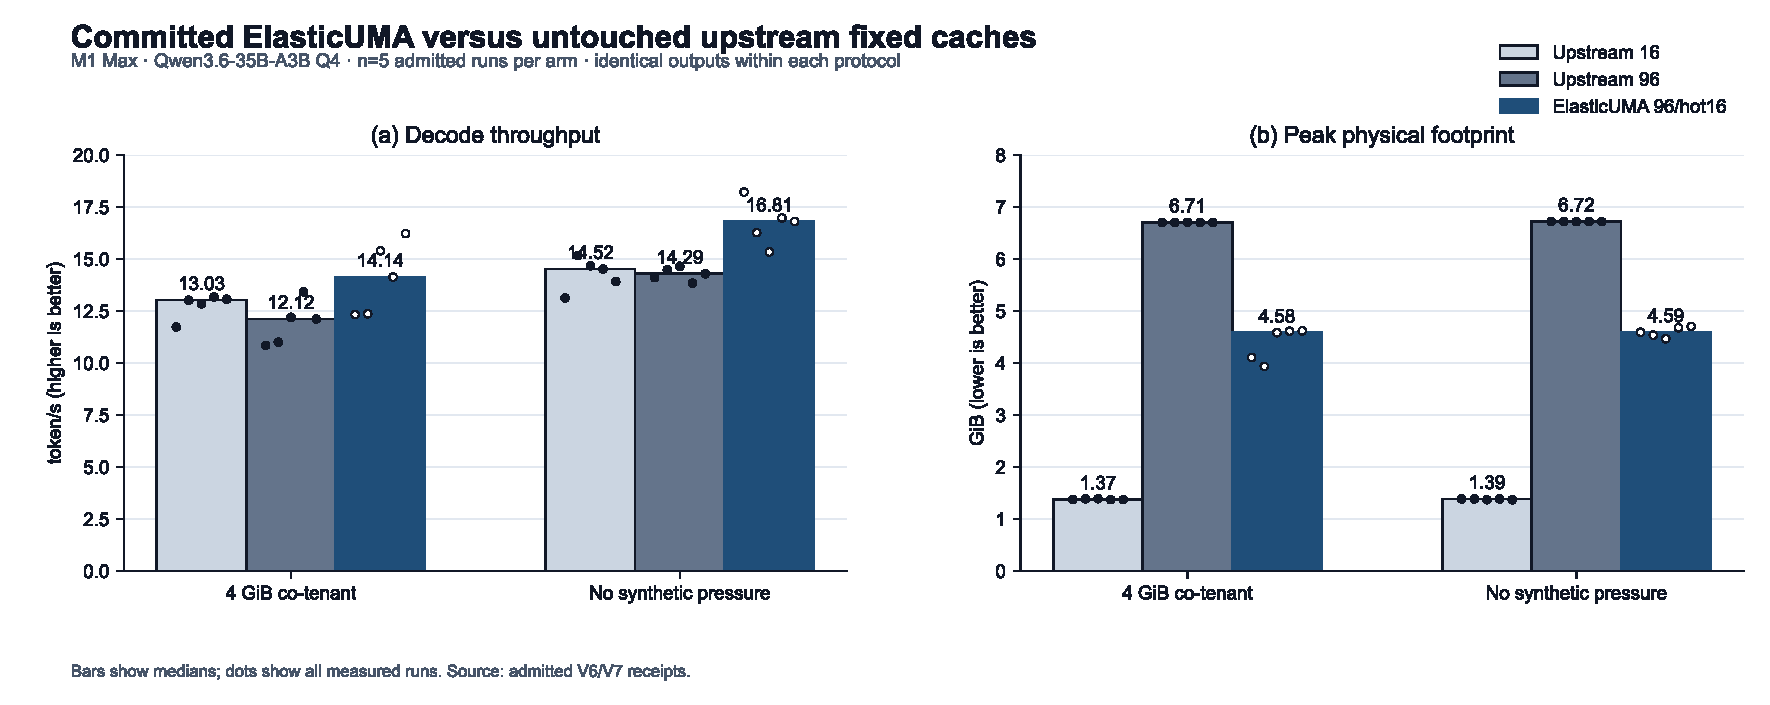
\includegraphics[width=0.98\linewidth]{figures/elasticuma-main-results.pdf}
  \caption{Qwen3.6 policy comparison. With the co-tenant, median throughput is
  14.136\tps for \system versus 13.025 and 12.116\tps for upstream-16 and
  upstream-96. Without it, the values are 16.807, 14.520, and 14.293\tps.
  Fixed-96 footprint falls by about one third under both protocols. Bars are arm
  medians; points are all measured runs.}
  \label{fig:qwen-main}
\end{figure}

\begin{figure}[tb]
  \centering
  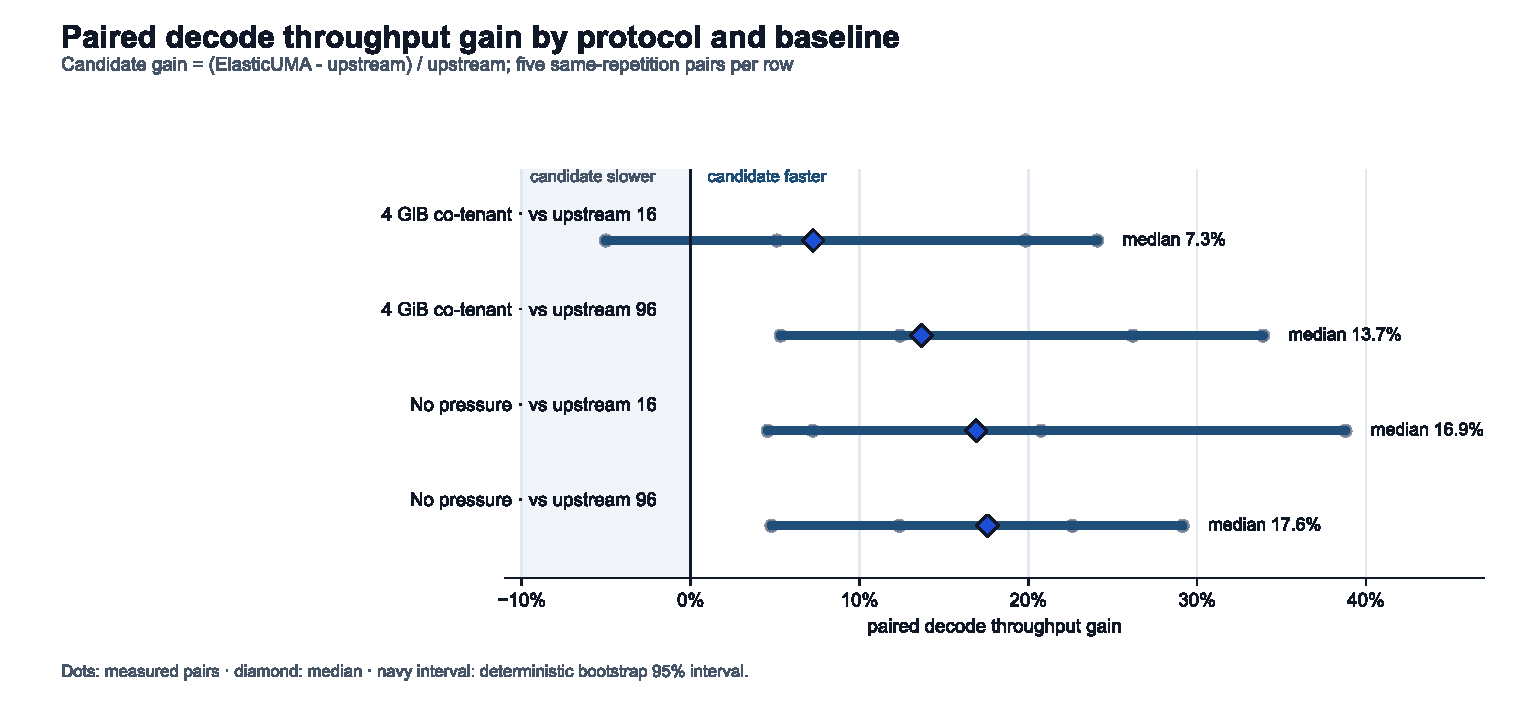
\includegraphics[width=0.90\linewidth]{figures/elasticuma-paired-gains.pdf}
  \caption{Matched Qwen decode gains against upstream-16 and upstream-96.
  Paired medians are 7.25\% and 13.67\% with the co-tenant and 16.91\% and
  17.59\% without it. Horizontal intervals are deterministic bootstrap 95\%
  intervals from five matched repetitions; the shaded region marks slowdowns.}
  \label{fig:paired}
\end{figure}

\subsection{RQ4: recovery is exercised, not inferred}

Every Qwen candidate row records volatile transitions, relocks, and a nonzero
empty-recovery count. Cumulative recovered bytes range from 9.090 to
10.758\,GiB per pressure-backed run and from 7.907 to 10.331\,GiB per
no-pressure run. These totals exceed instantaneous footprint because a cold
slot can be reclaimed and reloaded repeatedly.

All policies within V6 produce one identical response hash; V7 produces a
second within-protocol hash. These matching hashes demonstrated response-text
equality under greedy decoding despite real empty recovery. The current upstream CLI does not
expose generated token IDs, so we do not claim token-ID equality. The evidence
is stronger than a no-reclamation test but narrower than a full numerical trace
comparison.

\FloatBarrier
\pagebreak[4]

\subsection{RQ5: transfer to Gemma 4}

\begin{table}[ht]
\centering
\caption{Gemma 4 second-architecture validation without a pressure worker.
Values are medians of five admitted measured runs per arm.}
\label{tab:gemma}
\small
\begin{tabular}{lrrrrr}
\toprule
Policy & \multicolumn{1}{c}{tok/s} & \multicolumn{1}{c}{Hit} &
\multicolumn{1}{c}{Footprint} & \multicolumn{1}{c}{Compressor} &
\multicolumn{1}{c}{Min free} \\
\midrule
Upstream-16 & 16.394 & 65.52\% & 1.986\,GiB & 0.000\,GiB & 69\% \\
Upstream-96 & 18.742 & 98.40\% & 8.538\,GiB & 5.114\,GiB & 50\% \\
\system-96/16 & \textbf{23.820} & 95.79\% & 5.527\,GiB & 1.073\,GiB & 55\% \\
\bottomrule
\end{tabular}
\end{table}

\FloatBarrier

Gemma changes layer count, expert count, tokenizer, routing, and per-slot size.
To test architecture transfer without tuning, we preserve the Qwen 96/16
residency policy. Against the pinned upstream-16 and upstream-96 policies
\cite{patel2026slipstream}, \system wins every matched comparison. Paired-median
gains versus upstream-16 and upstream-96 are 45.30\% (interval 23.45--51.44\%)
and 26.01\% (interval 11.88--28.55\%), respectively. Relative to fixed-96, peak
footprint falls 35.26\%, from 8.538 to 5.527\,GiB; compressor growth falls from
5.114 to 1.073\,GiB. Hit rate remains 30.28 percentage points above the small
cache. All candidate rows exercise exact empty recovery (2.421--2.868\,GiB of
cumulative reload traffic), and no row grows swap.

\FloatBarrier

\begin{figure}[ht]
  \centering
  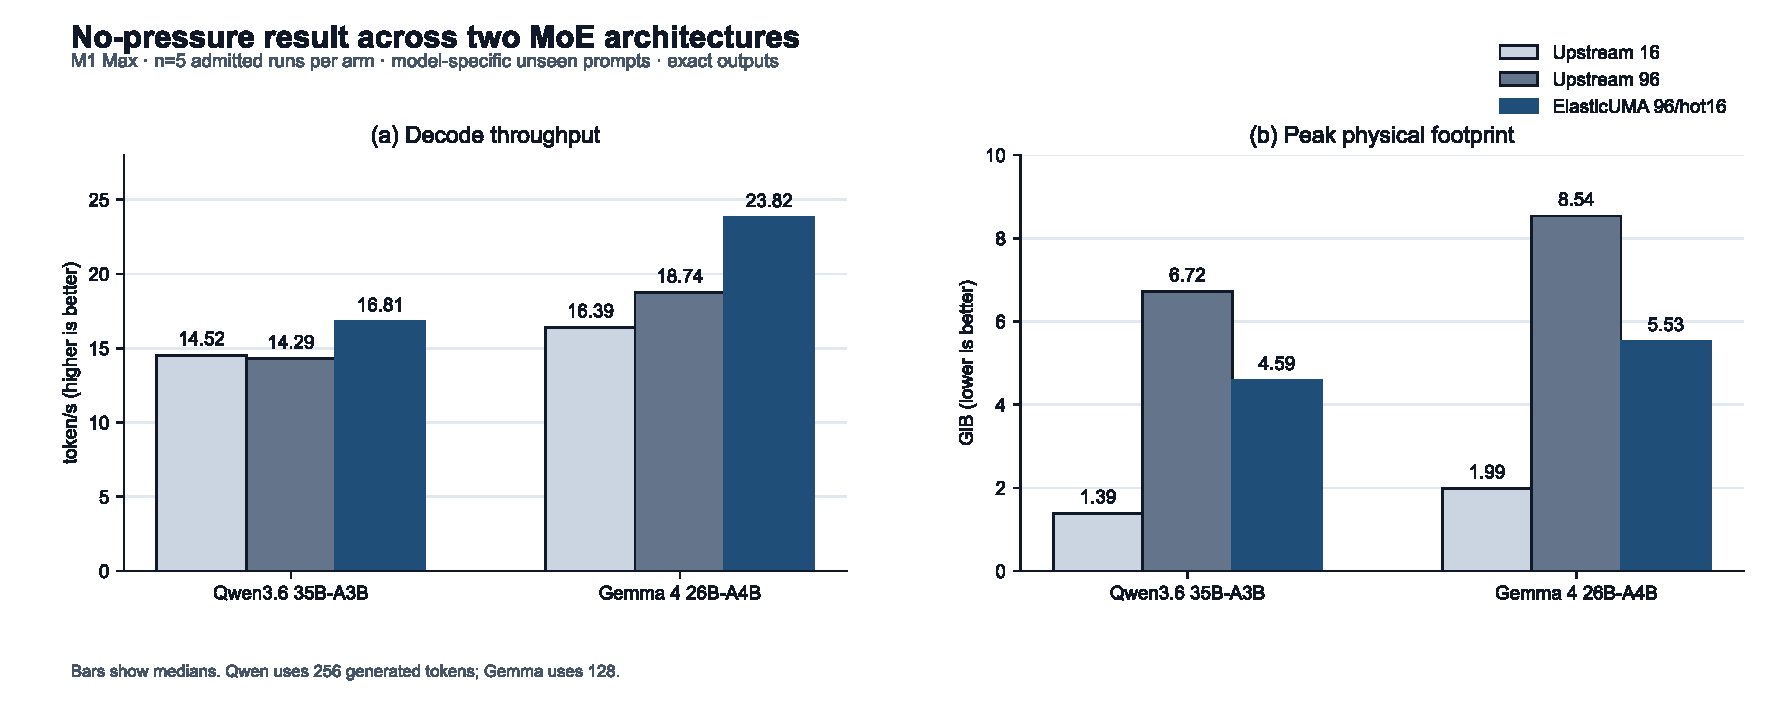
\includegraphics[width=0.98\linewidth]{figures/elasticuma-cross-model.pdf}
  \caption{No-pressure results across two MoE architectures. Absolute token
  rates are not a cross-model benchmark because prompts and generation lengths
  differ. Within each model, \system has the highest median decode rate and a
  materially lower footprint than upstream-96.}
  \label{fig:cross-model}
\end{figure}

\FloatBarrier

\subsection{Rejected alternatives and mechanism ablation}

\Cref{tab:ablations} records the measured failure criterion for each rejected
mechanism. This is a mechanism-screening record, not a quantitative aggregate
across incompatible prototypes.

\begin{table}[ht]
\centering
\caption{Alternatives rejected before the final per-slot, layerwise design.}
\label{tab:ablations}
\begin{tabularx}{0.98\linewidth}{>{\bfseries}l X}
\toprule
Alternative & Observed failure \\
\midrule
\code{F\_NOCACHE} & Advice changed file-cache treatment but did not release the anonymous slot allocation. \\
Direct mmap & Reduced measured model RSS from 3.38 to 1.92\,GiB in a probe, but was approximately 24 times slower than the cached positional-read path. \\
Raw/compressed MTLIO & Direct-storage variants missed frozen latency gates; lossless CPU decode reached only 0.46--2.85\,GiB/s. \\
One arena per layer & Coarse purgeability collapsed Qwen effective hit rate to 1.3\% and roughly halved throughput. \\
Post-prefill-only policy & Correctly marked cold slots but ran after the full cache had already materialized, failing the footprint gate. \\
\bottomrule
\end{tabularx}
\end{table}

\FloatBarrier

Only Metal-owned per-expert buffers, selective hot/cold state, and transitions
inside the synchronized layer loop satisfy both validity and footprint gates.

\subsection{Dense Qwen3.8 diagnostic}

We also run one canonical Qwen3.8-27B Q4 dense checkpoint with MLX
\cite{apple2026mlx}. One warmup and one 128-token measured row complete at
11.36\tps. The sampled peak physical footprint is 17.96\,GiB; MLX reports
18.60\,GiB peak memory. Minimum free memory reaches 20\%, and swap grows by
151\mib. A later row reaches
19\% free memory and is terminated by the frozen guard. Because the planned
five measured rows do not complete, this diagnostic is not admitted. We do not
use it as a speed, quality, or dense-versus-MoE comparison.

\FloatBarrier

\section{Discussion}
\label{sec:discussion}

\subsection{Why fewer physically entitled pages can be faster}

\system does not make SSD reads free and does not eliminate expert misses. Its
Qwen hit rate remains near 87\%, below fixed-96 near 91\% and far above
fixed-16 near 49\%. The improvement comes from a different system balance. The
large logical cache still captures reuse when cold pages survive, while the OS
can reclaim cold pages instead of compressing them or displacing more useful
file-backed state. The fixed-96 baseline shows that maximizing hit rate can
reduce service rate once its physical claim harms the shared pool.

This interpretation is supported by three observations. First, physical
footprint and compressor growth fall materially relative to fixed-96. Second,
the candidate leads in no-pressure experiments as well as under the controlled
co-tenant, so the result is not solely an artifact of one pressure process.
Third, repeated empty recovery occurs in every candidate row without output
divergence. The mechanism is therefore exercised in the measured path rather
than acting as an unused safety annotation.

\subsection{The OS as eviction partner, not model scheduler}

A recent kernel-cache study finds that ordinary OS replacement can be a strong
expert tier when the kernel sees the complete physical workload
\cite{si2026kernelcache}. \system reaches a related design point without
delegating model identity or exact publication to the kernel. The runtime
decides which pages are eligible, retains hot experts, validates slot contents,
and reloads exact weights. macOS decides whether eligible pages should remain
physical given global demand. This division avoids a runtime-only estimate of
desktop competition while preserving model-specific correctness.

The design is not a complete adaptive memory controller. It uses a fixed
logical/hot split and lets the OS react within the cold set. That simplicity is
a strength of the current evidence: there is no learned predictor, online
exploration, or second model configuration that can perturb the state being
measured. Future work can adapt the hot-set size, but it must beat this
non-destructive baseline and account for transition cost.

\subsection{Relationship to discrete-GPU edge serving}

FreeToken treats CPU memory, GPU memory, PCIe bandwidth, and CPU compute as
heterogeneous resources and continuously maps work across them
\cite{yang2026freetoken}. \system adopts its challenge-driven systems
discipline but not its CUDA data plane. On Apple Silicon there is no expert copy
across a host/device boundary. The relevant elasticity is whether cold shared
pages remain physically valid. CPU execution, bandwidth-adaptive miss splitting,
semantic checkpoints, and agent lifecycle management remain complementary.

\subsection{Implications for model support}

The mechanism transfers from Qwen's 256-expert, 40-layer layout to Gemma's
128-expert, 30-layer layout without policy tuning. That supports an
architecture-independent cache-validity abstraction, not arbitrary-model
compatibility. A new model still needs a correct tokenizer, packed manifest,
tensor mapping, router semantics, quantization decoder, and Metal kernels.
\system's public catalog makes checkpoint metadata data-driven, while the
native runtime remains the correctness boundary.

\subsection{Practical deployment}

The public CLI defaults to OS-managed 96/16 residency for admitted profiles and
offers one-shot generation plus a loopback OpenAI/Anthropic-shaped server. It
reuses one canonical model store, pins revisions, serializes downloads, and
refuses a transfer that would violate its disk reserve. These product surfaces
are engineering contributions for reproducibility and adoption; they are not
part of the measured algorithmic claim.

\section{Related Work}
\label{sec:related}

\subsection{Edge MoE serving and expert caching}

Edge MoE systems exploit sparsity through different resource assignments.
FreeToken co-designs residency, prefill streaming, CPU-GPU miss execution, and
elastic VRAM management for heterogeneous CUDA machines
\cite{yang2026freetoken}, whereas KTransformers moves selected MoE work to CPUs
and optimizes the hybrid path \cite{chen2025ktransformers}. MoE-Infinity instead
uses request-level activation traces to guide prefetching and caching on
personal machines \cite{xue2024moeinfinity}. Taken together, these systems
establish sparse local execution, but their main physical boundary is host
versus device memory; they do not control the lifetime of explicit Metal slot
pages inside one shared Apple pool.

MawForge stores full MoE weights on disk and materializes routed experts into a
bounded cache on unified-memory machines \cite{opie2026mawforge}, while
slipstream supplies native Metal execution, packed storage, positional reads,
and the fixed-cache baseline used here \cite{patel2026slipstream}. MawForge's
cache-size result motivates an end-to-end memory view; slipstream isolates the
residency mechanism under otherwise identical execution. Their shared
limitation is that a stable expert slot has no validity protocol after the OS
may discard its physical contents. \system does not claim their storage,
Metal, or LFU mechanisms as new.

\subsection{Representation and transfer reduction}

SliceMoE expands effective cache capacity through bit-sliced reconstruction
\cite{choi2026slicemoe}, whereas ZipMoE combines lossless expert compression
with cache-affinity scheduling \cite{yang2026zipmoe}. ExactMoE focuses on exact
low-bit slots and fused kernels \cite{saab2026exactmoe}. Despite changing
different parts of the representation and transfer path, all three leave a
separate residency question: a compressed, sliced, or fused cold slot still
needs a validity rule if its physical pages may disappear.
Overall, representation savings and residency validity are complementary rather
than competing solutions.

\subsection{Apple execution engines}

BaseRT improves native Metal kernels and dispatch
\cite{rathnayaka2026basert}, while FusionML identifies the eager boundary that
enables CPU-GPU prefill co-execution and the bandwidth limit that prevents a
similar decode benefit \cite{mohite2026fusionml}. NPUMoE maps static work to the
Apple Neural Engine but keeps CPU/GPU fallbacks for dynamic operations
\cite{benazir2026npumoe}. Collectively, these systems optimize where or how
computation runs. \system changes neither placement nor kernel math; it defines
a reload-correct, OS-discardable lifetime around the existing Metal path.

\subsection{Memory-aware runtimes and kernel ownership}

PagedAttention separates logical KV state from physical allocation to reduce
fragmentation \cite{kwon2023pagedattention}, while MemSpec coordinates draft
selection with resident memory on edge devices \cite{kim2026memspec}. By
contrast, the kernel-managed expert-cache study delegates replacement to the
page cache and finds that it can rival model-specific frequency policies under
equal limits \cite{si2026kernelcache}. \system follows the shared separation
principle but adds Metal-resource validity, GPU-safe transitions, and exact
reload for weights that retain stable logical slots.
Overall, these runtimes separate logical state from physical placement at
different layers; routed Metal weights add a validity transition that they do
not cover.

\subsection{Novelty boundary}

No individual component is claimed in isolation: expert caching, storage-backed
weights, Metal inference, LFU ranking, OS page replacement, and purgeable
graphics resources all predate this work. The contribution is their
reload-correct composition at per-expert granularity and real inference phase
boundaries, plus evidence that the composition improves the measured
throughput-footprint frontier against untouched fixed policies.

Across these categories, a specific gap remains among the cited systems: none
evaluates per-expert Metal resources that macOS may reclaim while their logical
cache identities survive, with relock-before-hit validation and exact recovery
at real inference boundaries. \system addresses that gap without claiming the
surrounding storage, caching, or Metal mechanisms as new.

\section{Limitations, Validity, and Ethics}
\label{sec:limitations}

\textbf{Hardware breadth.} All positive evidence comes from one 24-GPU-core M1
Max with 32\,GiB memory. Qwen and Gemma provide architectural diversity on the
same host, not cross-generation evidence. M2 through later Apple generations
may expose different memory, GPU, and purgeability behavior.

\textbf{Workload breadth.} Experiments use batch size one, short held-out
prompts, one 4,096-token context limit, and one controlled 4\,GiB co-tenant.
Real desktop traces, longer contexts, concurrent requests, multimodal inputs,
and tool-heavy sessions remain unevaluated. Qwen and Gemma use different prompts
and generation lengths, so cross-model absolute token rates are not comparable.

\textbf{Measurement.} macOS pressure events and compressor statistics are
system-wide and coarse. Physical footprint is process-specific and is the
primary memory metric, but it does not identify every causal path. Energy and
GPU power are unmeasured. Five matched repetitions support descriptive
bootstrap intervals, not population-level inference.

\textbf{Exactness.} Within-protocol response text is identical under greedy
decoding, and every candidate row exercises empty recovery. The pinned CLI does
not expose token IDs or per-layer numerical traces. We therefore avoid claims
of bitwise intermediate equality or model-quality improvement.

\textbf{Baselines.} The controlled baselines are the untouched fixed policies
of the same native runtime. This isolates the mechanism but does not establish
superiority over every version of MLX, llama.cpp, BaseRT, or another Mac engine.
Cross-runtime comparisons require matched model bytes, quantization, prompts,
context, output semantics, and memory accounting.

\textbf{Artifact and privacy.} The public artifact excludes model weights,
credentials, serial numbers, UUIDs, personal paths, and unrelated process
commands. Model checkpoints retain their own licenses and acceptable-use terms.
The loopback API has no authentication or TLS and must not be exposed to a LAN
or WAN. AI assistance is disclosed rather than treated as an anonymous author;
the named author remains responsible for verification and submission policy.

\section{Conclusion}
\label{sec:conclusion}

Our experiments demonstrate that a fixed expert cache equates logical capacity
with permanent physical entitlement. That assumption is costly on Apple unified memory, where model
slots, file-backed pages, GPU work, applications, compression, and swap share
one pool. \system separates the two. It preserves a large logical cache, offers
cold Metal-owned pages to macOS at GPU-safe boundaries, and converts every
discarded provisional hit into an exact reload.

On one M1 Max, the committed mechanism improves median decode throughput over
both small and large fixed upstream policies for Qwen3.6 and Gemma 4 while
reducing the large cache's peak physical footprint by roughly one third. The
contribution is the demonstrated separation of cache identity from physical
entitlement with exact recovery under real OS reclamation. The
negative precursor, failed alternatives, and incomplete dense control remain
part of the evidence record. The result is a systems mechanism scoped to the
tested host and workloads. The practical implication is that an Apple runtime
can retain cache identity without insisting that all cold pages remain physical.
The next decisive steps are independent
cross-generation reproduction, energy measurement, longer and concurrent
workloads, and comparison with strong external Mac runtimes under matched model
semantics.


\section*{Artifact Availability}
The public repository linked on the first page contains the user-facing source,
exact upstream patch, paper source, and analysis implementation. To keep that
repository focused, raw and admitted experiment receipts are distributed as a
separate companion release asset, \code{elasticuma-paper-v1.tar.gz}. The archive
has internal SHA-256 checksums and contains the evidence used to derive every
reported table and quantitative figure. Model weights, credentials, machine
identifiers, and local paths are excluded. Model checkpoints must be obtained
from their original publishers under their own licenses.

\begin{center}
\small
\begin{tabularx}{0.96\linewidth}{>{\bfseries\raggedright\arraybackslash}p{3.25cm} >{\raggedright\arraybackslash}X}
\toprule
Artifact layer & Public location \\
\midrule
Runtime mechanism & \code{runtime/patches/} and \code{scripts/bootstrap\_candidate\_runtime.sh} \\
User software & \code{src/elasticuma/}, \code{install.sh}, and the public documentation \\
Measured evidence & Companion release asset \code{elasticuma-paper-v1.tar.gz} \\
Analysis and figures & Evidence archive plus \code{paper/latex/figures/} \\
Paper source & \code{paper/latex/}, including the bibliography and vector figures \\
\bottomrule
\end{tabularx}
\end{center}

The separate archive retains negative results and failed alternatives in the
same evidence lineage as admitted results. Reproductions that disagree with the
reported measurements should be retained rather than tuned away.

\section*{Acknowledgments and Disclosure}
The author thanks the maintainers of slipstream, MLX, llama.cpp, and FreeToken
for publishing code and documentation that made direct comparison possible.
AI-assisted tools supported implementation, experiment orchestration, figure
generation, and editorial revision. The named author selected the research
questions, reviewed the source and prior art, verified the measurements and
claims, and accepts responsibility for the manuscript and released artifacts.

\renewcommand{\bibfont}{\small\raggedright}
\setlength{\bibsep}{3pt plus 1pt minus 1pt}
\bibliographystyle{unsrtnat}
\bibliography{references}

\end{document}
